\input{formats/presentation.tex}

\usepackage{adjustbox}
\usepackage{amsfonts}
\title[Курсовая работа]
    {Построение параллельных алгоритмов для решения задачи быстродействия с фазовыми ограничениями}
\author[К. Ю. Егоров]
    {студент 5 курса К. Ю. Егоров\\
    научный руководитель --- к.ф-м.н., доцент И. В. Востриков}
\institute{Кафедра системного анализа}
\date{28 мая 2022 г.}

\begin{document}
    \maketitle
    \begin{frame}[t]{Постановка задачи}
        Рассмотрим задачу
        \begin{equation*}
            \dot x = f(t,x,u),\;\mbox{где $x = [x_1, x_2, \dot x_1, \dot x_2]$.}
        \end{equation*}
        Фазовые ограничения
        \begin{equation*}
            [x_1, x_2] \in \Omega \subseteq \mathbb{R}^2.
        \end{equation*}
        Минимизируем функционал
        \begin{equation*}
            J(u) = \int_{t_0}^{t_1}g(x, u)\,dt \to \min_u.
        \end{equation*}
        Необходимо решать уравнение Гамильтона--Якоби--Беллмана
        \begin{equation*}
            \min\limits_{u \in U}\left\{
                g(x,u) + \sum\limits_{i=1}^{n}\frac{\partial V(x)}{\partial x_i} f_i(x,u)
            \right\} = 0.
        \end{equation*}
    \end{frame}
    \begin{frame}[t]{Дискретизация задачи}
        Введем равномерную сетку
        \begin{equation*}
            \Xi = \left\{ (x_i , y_j) \in \Pi , x_i = \varepsilon\frac{i}{N} , y_j = \varepsilon\frac{j}{M} \right\},\,
            \mbox{где $\Omega \subseteq \Pi$}.
        \end{equation*}
        Возможные переходы для $(i,j)$
        \begin{equation*}
            \mathrm{possible}(i,j) = \{
                (i, j) \;|\; i \in \{i, i \pm 1\}, j \in \{j, j \pm 1\}, (x_i,y_j) \in \Omega    
            \}
        \end{equation*}
        \textit{Предложение.} Время перехода не зависит от предыдущей скорости и направления. Обозначим это время за
        \begin{equation*}
            d_{i_{from},\,j_{from}}(i_{to},\,j_{to}).
        \end{equation*}
        Неявное матричное уравнение
        \begin{equation*}
            \begin{aligned}
                &V_{i,j} = \min\limits_{(\hat i,\,\hat j) \in \mathrm{possible}(i,\,j)}\{d_{i,\,j}(\hat i,\,\hat j) + V_{\hat i,\,\hat j}\}, \\
                &V_{i_1,\,j_1} = 0.
            \end{aligned}
        \end{equation*}
    \end{frame}
    \begin{frame}[t]{Алгоритм Беллмана--Форда}
        \begin{enumerate}
            \item Изначально все узлы, кроме целевого, промаркированы значением $+\infty$, а целевой~--- нулем;
            \item Необходимо провести $(NM - 1)$ итерации алгоритма;
            \item На каждой итерации происходит полный проход по сетке, далее $(i,j)$ --- позиция при проходе;
            \item Для каждой вершины из возможного множества $(\hat i, \hat j) \in \mathrm{possible}(i,j)$ происходит перемаркировка: в случае, если $V(i, j) > d_{i,j}(\hat i, \hat j) + V(\hat i, \hat j)$, перемаркируем
            \[
                V(i,j) \leftarrowtail d_{i,j}(\hat i, \hat j) + V(\hat i, \hat j).
            \]
        \end{enumerate}
        \begin{block}{Замечание}
            Оптимальная траектория не может иметь более $(NM - 1)$ перемещения. Таким образом алгоритм действительно ищет кратчайший путь.
        \end{block}
    \end{frame}
    \begin{frame}[t]{Параллельный алгоритм Беллмана--Форда}
        На центральном процессоре
        \begin{itemize}
            \item Разбиваем сетку на каждой итерации на $C$ (число ядер) подсеток, считающихся параллельно
            \item Синхронизацию при обработке последнего ряда подсетки осуществляем массивом мьютексов
        \end{itemize}
        На графическом процессоре
        \begin{itemize}
            \item Каждый узел считается на отдельном процессоре
            \item Синхронизация осуществляется за счет того, что проводится не один проход по матрице, а восемь: отдельно для каждого возможного направления движения
        \end{itemize}
        На многонодной установке
        \begin{itemize}
            \item Одна мастер программа, $LC_l$ (совокупное число ядер) вычислителей (сервисов, общающихся по http)
            \item Синхронизация осуществляется за счет передачи мастером минимального инкремента каждому вычислителю
        \end{itemize}
    \end{frame}
    \begin{frame}[t]{Алгоритм Дейкстры}
        \begin{enumerate}
            \item На начало алгоритма в множестве граничных узлов находится только целевой узел. 
            \item На каждой итерации алгоритма из множества граничных узлов выбирается узел с минимальной маркировкой.
            \item Этот узел добавляется в множество обработанных узлов и удаляется из граничного множества.
            \item Затем из возможного множества выбираются узлы, которые не находятся в множестве обработанных узлов. Эти узлы добавляются в множество граничных вершин, маркировка таких вершин обновляется.
        \end{enumerate}
        Алгоритм останавливается в случае, если на некоторой итерации алгоритма был выбран начальный узел $(i_0,j_0)$.
    \end{frame}
    \begin{frame}[t]{Параллельный алгоритм Дейкстры}
        Распараллеливанию подвергается самый алгоритмически сложная часть алгоритма~--- поиск минимума в граничном множестве. Для этого граничное множество представляется в виде $C$ (число доступных ядер процессора) хэш-таблиц. Запись нового узла осуществляется в наименее полную таблицу.

        \begin{itemize}
            \item Для программы на центральном процессоре не требуется дополнительная синхронизация;
            \item Нет нативного метода, который мог бы поддержать графический процессор, так как взаимодействие с ним осуществляется копированием последовательных страниц памяти. Это потребовало бы использование массива для хранения граничного множества, и в конечном итоге ускорение было бы скомпенсировано операцией удаления из массива;
            \item Для многонодной установки минимальная инкрементальная информация~--- это выбранный узел, и узлы, добавленные в граничное множество.
        \end{itemize}
    \end{frame}
    \begin{frame}[t]{Программное решение}
        Программы написаны на языке Go
        \begin{itemize}
            \item go routines;
            \item компилируемый;
            \item сборка мусора.
        \end{itemize}
        Помимо основных алгоритмов написаны:
        \begin{itemize}
            \item генератор ландшафта, использующий перлиновый шум;
            \item визуализатор пути, использующий OpenGL.
        \end{itemize}
        Программы для многонодной установки
        \begin{itemize}
            \item поставляются в виде двух docker-образов: для мастера и вычислителе;.
            \item тестировалось только на Kubernetes кластере;
            \item требуют ручного применения Kubernetes манифестов.
        \end{itemize}
    \end{frame}
    \begin{frame}[t]{Пример 1}
        Алгоритм Дейкстры из $(1,\,1)$ в $(1000,\,1000)$
        \begin{center}
            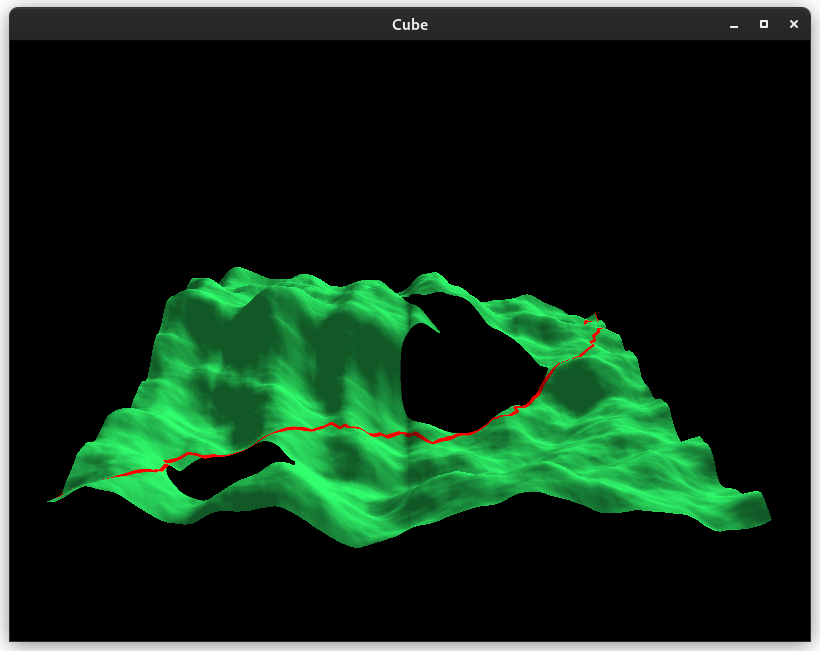
\includegraphics[scale=0.18]{content/dijkstra.png}
            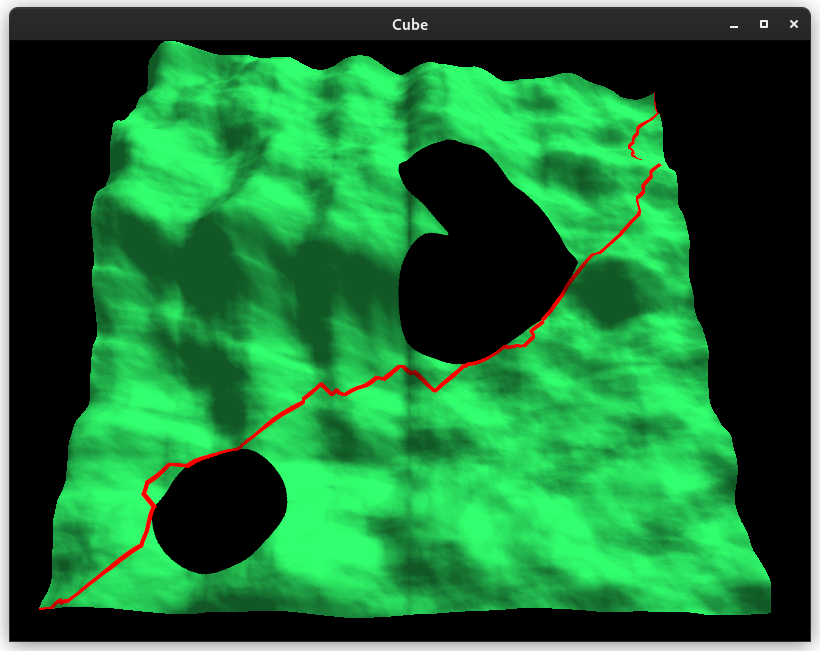
\includegraphics[scale=0.18]{content/dijkstra-top.png}
        \end{center}
        Время перехода
        \[
            d_{i,j}(\hat i, \hat j) = 100\cdot(\mathrm{height}(\hat i, \hat j) - \mathrm{height}(i, j))_{+} + 5.
        \]
    \end{frame}
    \begin{frame}[t]{Пример 2}
        Алгоритм Беллмана--Форда из $(1,\,1)$ в $(90,\,90)$
        \begin{center}
            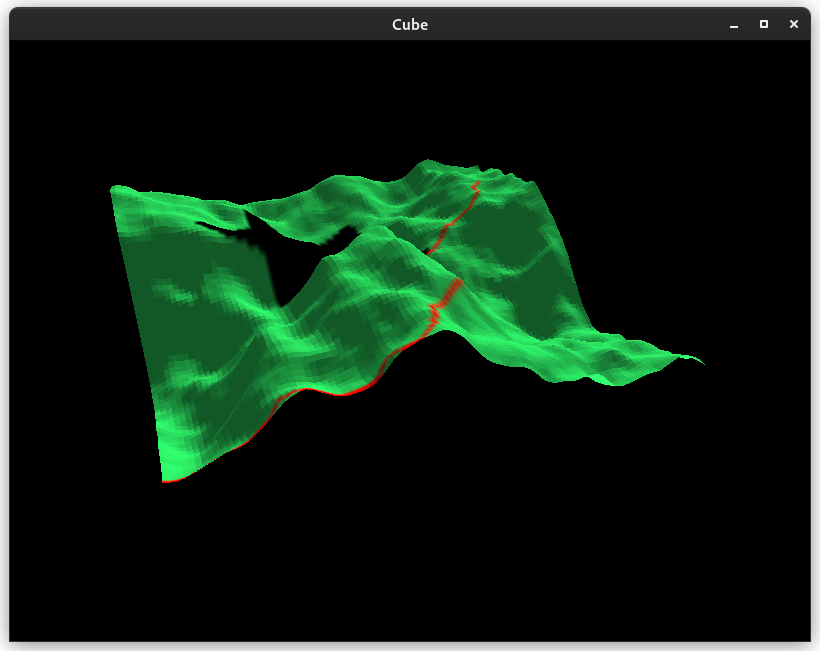
\includegraphics[scale=0.18]{content/bf.png}
            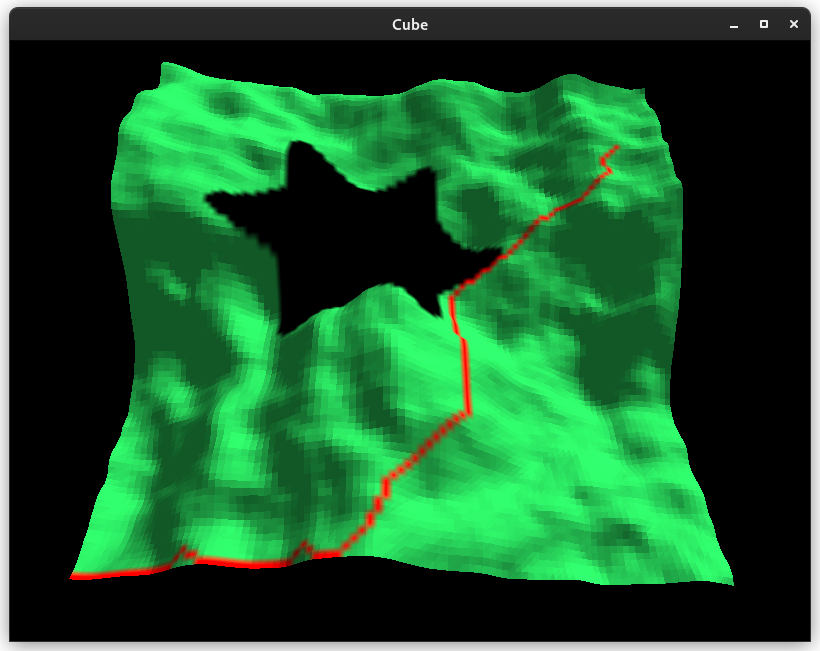
\includegraphics[scale=0.18]{content/bf-top.png}
        \end{center}
        Время перехода
        \[
            d_{i,j}(\hat i, \hat j) = 100\cdot(\mathrm{height}(\hat i, \hat j) - \mathrm{height}(i, j))_{+} + 5.
        \]
    \end{frame}
    \begin{frame}[t]{Сравнение времени работы}
        Время работы алгоритма Беллмана--Форда
            \begin{tabular}{ | l | l | l | l |}
                \hline
                Сетка   & Классический    & Парал. однонод. & Парал. многонод. \\ \hline
                50$\times$50   & 2s              & 700ms             & 2s                 \\
                100$\times$100 & 28s             & 11s               & 24s                \\
                250$\times$250 & 14m 17s         & 4m 56s            & 10m 24s             \\
                500$\times$500 & $\approx$4h 50m & $\approx$1h 20m   & $\approx$2h 40m    \\
                \hline
            \end{tabular}
        \vfill 
        Время работы алгоритма Дейкстры
            \begin{tabular}{ | l | l | l | l |}
                \hline
                Сетка     & Классический    & Парал. однонод. & Парал. многонод. \\ \hline
                500$\times$500   & 2.9             & 4.5s              & 19.4s               \\
                1000$\times$1000 & 36s             & 40s               & 3m 20s             \\
                2500$\times$2500 & 10m 40s         & 6m 48s            & 34m 42s            \\
                5000$\times$5000 & $\approx$1h 15m & $\approx$39m      & $\approx$2h 40m    \\
                \hline
            \end{tabular}
    \end{frame}
    \begin{frame}[t]{Литература}
        \begin{enumerate}
            \item Беллман~Р., Дрейфус~С. \textit{Прикладные задачи динамического программирования.} М.:~Наука,~1965.
            \item Shu-Xi, Wang. \textit{The Improved Dijkstra's Shortest Path Algorithm and Its Application.} Procedia Engineering. 29. 1186-1190. 2012.
            \item Glabowski, M., Musznicki, B. \textit{Review and Performance Analysis of Shortest Path Problem Solving Algorithms.} International Journal On Advances in Software. 7. 20-30. 2014.
            \item Ведякова А. О., Милованович Е. В. \textit{Методы теории оптимального управления.} М.: Редакционно-издательский отдел Университета ИТМО. Санкт-Петербург, 2021.
        \end{enumerate}
    \end{frame}
\end{document}

\usepackage{adjustbox}
\usepackage{amsfonts}
\title[Курсовая работа]
    {Построение параллельных алгоритмов для решения задачи быстродействия с фазовыми ограничениями}
\author[К. Ю. Егоров]
    {студент 5 курса К. Ю. Егоров\\
    научный руководитель --- к.ф-м.н., доцент И. В. Востриков}
\institute{Кафедра системного анализа}
\date{28 мая 2022 г.}

\begin{document}
    \maketitle
    \begin{frame}[t]{Постановка задачи}
        Рассмотрим задачу
        \begin{equation*}
            \dot x = f(t,x,u),\;\mbox{где $x = [x_1, x_2, \dot x_1, \dot x_2]$.}
        \end{equation*}
        Фазовые ограничения
        \begin{equation*}
            [x_1, x_2] \in \Omega \subseteq \mathbb{R}^2.
        \end{equation*}
        Минимизируем функционал
        \begin{equation*}
            J(u) = \int_{t_0}^{t_1}g(x, u)\,dt \to \min_u.
        \end{equation*}
        Необходимо решать уравнение Гамильтона--Якоби--Беллмана
        \begin{equation*}
            \min\limits_{u \in U}\left\{
                g(x,u) + \sum\limits_{i=1}^{n}\frac{\partial V(x)}{\partial x_i} f_i(x,u)
            \right\} = 0.
        \end{equation*}
    \end{frame}
    \begin{frame}[t]{Дискретизация задачи}
        Введем равномерную сетку
        \begin{equation*}
            \Xi = \left\{ (x_i , y_j) \in \Pi , x_i = \varepsilon\frac{i}{N} , y_j = \varepsilon\frac{j}{M} \right\},\,
            \mbox{где $\Omega \subseteq \Pi$}.
        \end{equation*}
        Возможные переходы для $(i,j)$
        \begin{equation*}
            \mathrm{possible}(i,j) = \{
                (i, j) \;|\; i \in \{i, i \pm 1\}, j \in \{j, j \pm 1\}, (x_i,y_j) \in \Omega    
            \}
        \end{equation*}
        \textit{Предложение.} Время перехода не зависит от предыдущей скорости и направления. Обозначим это время за
        \begin{equation*}
            d_{i_{from},\,j_{from}}(i_{to},\,j_{to}).
        \end{equation*}
        Неявное матричное уравнение
        \begin{equation*}
            \begin{aligned}
                &V_{i,j} = \min\limits_{(\hat i,\,\hat j) \in \mathrm{possible}(i,\,j)}\{d_{i,\,j}(\hat i,\,\hat j) + V_{\hat i,\,\hat j}\}, \\
                &V_{i_1,\,j_1} = 0.
            \end{aligned}
        \end{equation*}
    \end{frame}
    \begin{frame}[t]{Алгоритм Беллмана--Форда}
        \begin{enumerate}
            \item Изначально все узлы, кроме целевого, промаркированы значением $+\infty$, а целевой~--- нулем;
            \item Необходимо провести $(NM - 1)$ итерации алгоритма;
            \item На каждой итерации происходит полный проход по сетке, далее $(i,j)$ --- позиция при проходе;
            \item Для каждой вершины из возможного множества $(\hat i, \hat j) \in \mathrm{possible}(i,j)$ происходит перемаркировка: в случае, если $V(i, j) > d_{i,j}(\hat i, \hat j) + V(\hat i, \hat j)$, перемаркируем
            \[
                V(i,j) \leftarrowtail d_{i,j}(\hat i, \hat j) + V(\hat i, \hat j).
            \]
        \end{enumerate}
        \begin{block}{Замечание}
            Оптимальная траектория не может иметь более $(NM - 1)$ перемещения. Таким образом алгоритм действительно ищет кратчайший путь.
        \end{block}
    \end{frame}
    \begin{frame}[t]{Параллельный алгоритм Беллмана--Форда}
        На центральном процессоре
        \begin{itemize}
            \item Разбиваем сетку на каждой итерации на $C$ (число ядер) подсеток, считающихся параллельно
            \item Синхронизацию при обработке последнего ряда подсетки осуществляем массивом мьютексов
        \end{itemize}
        На графическом процессоре
        \begin{itemize}
            \item Каждый узел считается на отдельном процессоре
            \item Синхронизация осуществляется за счет того, что проводится не один проход по матрице, а восемь: отдельно для каждого возможного направления движения
        \end{itemize}
        На многонодной установке
        \begin{itemize}
            \item Одна мастер программа, $LC_l$ (совокупное число ядер) вычислителей (сервисов, общающихся по http)
            \item Синхронизация осуществляется за счет передачи мастером минимального инкремента каждому вычислителю
        \end{itemize}
    \end{frame}
    \begin{frame}[t]{Алгоритм Дейкстры}
        \begin{enumerate}
            \item На начало алгоритма в множестве граничных узлов находится только целевой узел. 
            \item На каждой итерации алгоритма из множества граничных узлов выбирается узел с минимальной маркировкой.
            \item Этот узел добавляется в множество обработанных узлов и удаляется из граничного множества.
            \item Затем из возможного множества выбираются узлы, которые не находятся в множестве обработанных узлов. Эти узлы добавляются в множество граничных вершин, маркировка таких вершин обновляется.
        \end{enumerate}
        Алгоритм останавливается в случае, если на некоторой итерации алгоритма был выбран начальный узел $(i_0,j_0)$.
    \end{frame}
    \begin{frame}[t]{Параллельный алгоритм Дейкстры}
        Распараллеливанию подвергается самый алгоритмически сложная часть алгоритма~--- поиск минимума в граничном множестве. Для этого граничное множество представляется в виде $C$ (число доступных ядер процессора) хэш-таблиц. Запись нового узла осуществляется в наименее полную таблицу.

        \begin{itemize}
            \item Для программы на центральном процессоре не требуется дополнительная синхронизация;
            \item Нет нативного метода, который мог бы поддержать графический процессор, так как взаимодействие с ним осуществляется копированием последовательных страниц памяти. Это потребовало бы использование массива для хранения граничного множества, и в конечном итоге ускорение было бы скомпенсировано операцией удаления из массива;
            \item Для многонодной установки минимальная инкрементальная информация~--- это выбранный узел, и узлы, добавленные в граничное множество.
        \end{itemize}
    \end{frame}
    \begin{frame}[t]{Программное решение}
        Программы написаны на языке Go
        \begin{itemize}
            \item go routines;
            \item компилируемый;
            \item сборка мусора.
        \end{itemize}
        Помимо основных алгоритмов написаны:
        \begin{itemize}
            \item генератор ландшафта, использующий перлиновый шум;
            \item визуализатор пути, использующий OpenGL.
        \end{itemize}
        Программы для многонодной установки
        \begin{itemize}
            \item поставляются в виде двух docker-образов: для мастера и вычислителе;.
            \item тестировалось только на Kubernetes кластере;
            \item требуют ручного применения Kubernetes манифестов.
        \end{itemize}
    \end{frame}
    \begin{frame}[t]{Пример 1}
        Алгоритм Дейкстры из $(1,\,1)$ в $(1000,\,1000)$
        \begin{center}
            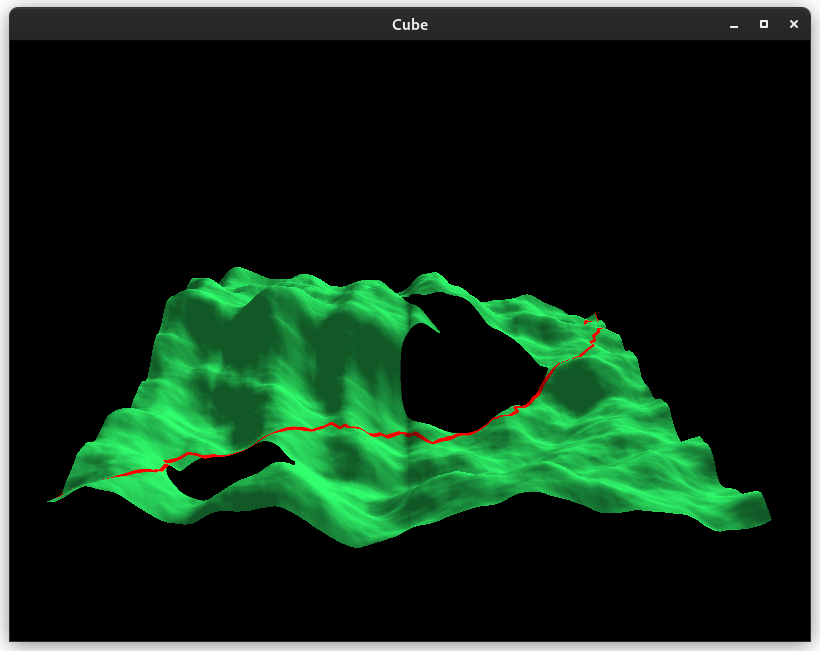
\includegraphics[scale=0.18]{content/dijkstra.png}
            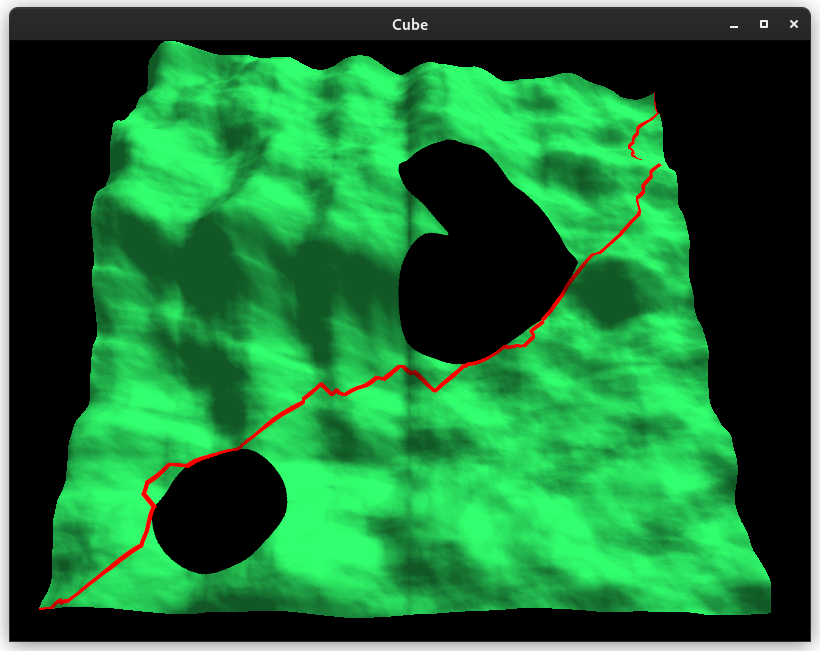
\includegraphics[scale=0.18]{content/dijkstra-top.png}
        \end{center}
        Время перехода
        \[
            d_{i,j}(\hat i, \hat j) = 100\cdot(\mathrm{height}(\hat i, \hat j) - \mathrm{height}(i, j))_{+} + 5.
        \]
    \end{frame}
    \begin{frame}[t]{Пример 2}
        Алгоритм Беллмана--Форда из $(1,\,1)$ в $(90,\,90)$
        \begin{center}
            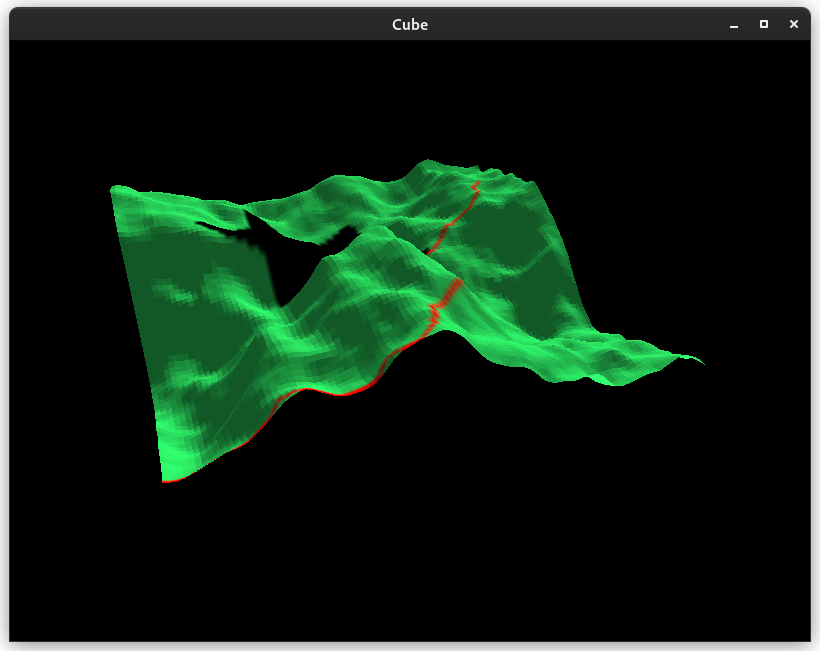
\includegraphics[scale=0.18]{content/bf.png}
            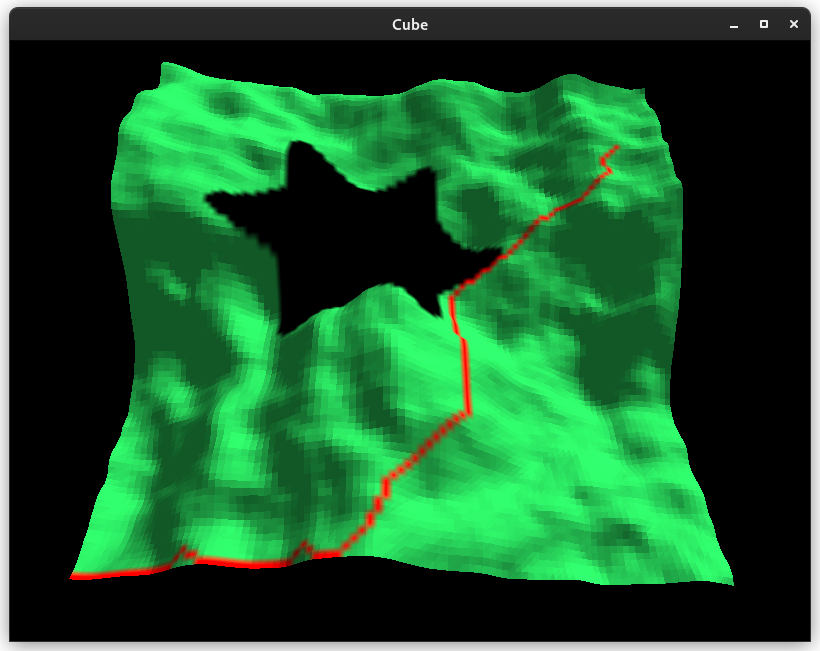
\includegraphics[scale=0.18]{content/bf-top.png}
        \end{center}
        Время перехода
        \[
            d_{i,j}(\hat i, \hat j) = 100\cdot(\mathrm{height}(\hat i, \hat j) - \mathrm{height}(i, j))_{+} + 5.
        \]
    \end{frame}
    \begin{frame}[t]{Сравнение времени работы}
        Время работы алгоритма Беллмана--Форда
            \begin{tabular}{ | l | l | l | l |}
                \hline
                Сетка   & Классический    & Парал. однонод. & Парал. многонод. \\ \hline
                50$\times$50   & 2s              & 700ms             & 2s                 \\
                100$\times$100 & 28s             & 11s               & 24s                \\
                250$\times$250 & 14m 17s         & 4m 56s            & 10m 24s             \\
                500$\times$500 & $\approx$4h 50m & $\approx$1h 20m   & $\approx$2h 40m    \\
                \hline
            \end{tabular}
        \vfill 
        Время работы алгоритма Дейкстры
            \begin{tabular}{ | l | l | l | l |}
                \hline
                Сетка     & Классический    & Парал. однонод. & Парал. многонод. \\ \hline
                500$\times$500   & 2.9             & 4.5s              & 19.4s               \\
                1000$\times$1000 & 36s             & 40s               & 3m 20s             \\
                2500$\times$2500 & 10m 40s         & 6m 48s            & 34m 42s            \\
                5000$\times$5000 & $\approx$1h 15m & $\approx$39m      & $\approx$2h 40m    \\
                \hline
            \end{tabular}
    \end{frame}
    \begin{frame}[t]{Литература}
        \begin{enumerate}
            \item Беллман~Р., Дрейфус~С. \textit{Прикладные задачи динамического программирования.} М.:~Наука,~1965.
            \item Shu-Xi, Wang. \textit{The Improved Dijkstra's Shortest Path Algorithm and Its Application.} Procedia Engineering. 29. 1186-1190. 2012.
            \item Glabowski, M., Musznicki, B. \textit{Review and Performance Analysis of Shortest Path Problem Solving Algorithms.} International Journal On Advances in Software. 7. 20-30. 2014.
            \item Ведякова А. О., Милованович Е. В. \textit{Методы теории оптимального управления.} М.: Редакционно-издательский отдел Университета ИТМО. Санкт-Петербург, 2021.
        \end{enumerate}
    \end{frame}
\end{document}

\usepackage{adjustbox}
\usepackage{amsfonts}
\title[Курсовая работа]
    {Построение параллельных алгоритмов для решения задачи быстродействия с фазовыми ограничениями}
\author[К. Ю. Егоров]
    {студент 5 курса К. Ю. Егоров\\
    научный руководитель --- к.ф-м.н., доцент И. В. Востриков}
\institute{Кафедра системного анализа}
\date{28 мая 2022 г.}

\begin{document}
    \maketitle
    \begin{frame}[t]{Постановка задачи}
        Рассмотрим задачу
        \begin{equation*}
            \dot x = f(t,x,u),\;\mbox{где $x = [x_1, x_2, \dot x_1, \dot x_2]$.}
        \end{equation*}
        Фазовые ограничения
        \begin{equation*}
            [x_1, x_2] \in \Omega \subseteq \mathbb{R}^2.
        \end{equation*}
        Минимизируем функционал
        \begin{equation*}
            J(u) = \int_{t_0}^{t_1}g(x, u)\,dt \to \min_u.
        \end{equation*}
        Необходимо решать уравнение Гамильтона--Якоби--Беллмана
        \begin{equation*}
            \min\limits_{u \in U}\left\{
                g(x,u) + \sum\limits_{i=1}^{n}\frac{\partial V(x)}{\partial x_i} f_i(x,u)
            \right\} = 0.
        \end{equation*}
    \end{frame}
    \begin{frame}[t]{Дискретизация задачи}
        Введем равномерную сетку
        \begin{equation*}
            \Xi = \left\{ (x_i , y_j) \in \Pi , x_i = \varepsilon\frac{i}{N} , y_j = \varepsilon\frac{j}{M} \right\},\,
            \mbox{где $\Omega \subseteq \Pi$}.
        \end{equation*}
        Возможные переходы для $(i,j)$
        \begin{equation*}
            \mathrm{possible}(i,j) = \{
                (i, j) \;|\; i \in \{i, i \pm 1\}, j \in \{j, j \pm 1\}, (x_i,y_j) \in \Omega    
            \}
        \end{equation*}
        \textit{Предложение.} Время перехода не зависит от предыдущей скорости и направления. Обозначим это время за
        \begin{equation*}
            d_{i_{from},\,j_{from}}(i_{to},\,j_{to}).
        \end{equation*}
        Неявное матричное уравнение
        \begin{equation*}
            \begin{aligned}
                &V_{i,j} = \min\limits_{(\hat i,\,\hat j) \in \mathrm{possible}(i,\,j)}\{d_{i,\,j}(\hat i,\,\hat j) + V_{\hat i,\,\hat j}\}, \\
                &V_{i_1,\,j_1} = 0.
            \end{aligned}
        \end{equation*}
    \end{frame}
    \begin{frame}[t]{Алгоритм Беллмана--Форда}
        \begin{enumerate}
            \item Изначально все узлы, кроме целевого, промаркированы значением $+\infty$, а целевой~--- нулем;
            \item Необходимо провести $(NM - 1)$ итерации алгоритма;
            \item На каждой итерации происходит полный проход по сетке, далее $(i,j)$ --- позиция при проходе;
            \item Для каждой вершины из возможного множества $(\hat i, \hat j) \in \mathrm{possible}(i,j)$ происходит перемаркировка: в случае, если $V(i, j) > d_{i,j}(\hat i, \hat j) + V(\hat i, \hat j)$, перемаркируем
            \[
                V(i,j) \leftarrowtail d_{i,j}(\hat i, \hat j) + V(\hat i, \hat j).
            \]
        \end{enumerate}
        \begin{block}{Замечание}
            Оптимальная траектория не может иметь более $(NM - 1)$ перемещения. Таким образом алгоритм действительно ищет кратчайший путь.
        \end{block}
    \end{frame}
    \begin{frame}[t]{Параллельный алгоритм Беллмана--Форда}
        На центральном процессоре
        \begin{itemize}
            \item Разбиваем сетку на каждой итерации на $C$ (число ядер) подсеток, считающихся параллельно
            \item Синхронизацию при обработке последнего ряда подсетки осуществляем массивом мьютексов
        \end{itemize}
        На графическом процессоре
        \begin{itemize}
            \item Каждый узел считается на отдельном процессоре
            \item Синхронизация осуществляется за счет того, что проводится не один проход по матрице, а восемь: отдельно для каждого возможного направления движения
        \end{itemize}
        На многонодной установке
        \begin{itemize}
            \item Одна мастер программа, $LC_l$ (совокупное число ядер) вычислителей (сервисов, общающихся по http)
            \item Синхронизация осуществляется за счет передачи мастером минимального инкремента каждому вычислителю
        \end{itemize}
    \end{frame}
    \begin{frame}[t]{Алгоритм Дейкстры}
        \begin{enumerate}
            \item На начало алгоритма в множестве граничных узлов находится только целевой узел. 
            \item На каждой итерации алгоритма из множества граничных узлов выбирается узел с минимальной маркировкой.
            \item Этот узел добавляется в множество обработанных узлов и удаляется из граничного множества.
            \item Затем из возможного множества выбираются узлы, которые не находятся в множестве обработанных узлов. Эти узлы добавляются в множество граничных вершин, маркировка таких вершин обновляется.
        \end{enumerate}
        Алгоритм останавливается в случае, если на некоторой итерации алгоритма был выбран начальный узел $(i_0,j_0)$.
    \end{frame}
    \begin{frame}[t]{Параллельный алгоритм Дейкстры}
        Распараллеливанию подвергается самый алгоритмически сложная часть алгоритма~--- поиск минимума в граничном множестве. Для этого граничное множество представляется в виде $C$ (число доступных ядер процессора) хэш-таблиц. Запись нового узла осуществляется в наименее полную таблицу.

        \begin{itemize}
            \item Для программы на центральном процессоре не требуется дополнительная синхронизация;
            \item Нет нативного метода, который мог бы поддержать графический процессор, так как взаимодействие с ним осуществляется копированием последовательных страниц памяти. Это потребовало бы использование массива для хранения граничного множества, и в конечном итоге ускорение было бы скомпенсировано операцией удаления из массива;
            \item Для многонодной установки минимальная инкрементальная информация~--- это выбранный узел, и узлы, добавленные в граничное множество.
        \end{itemize}
    \end{frame}
    \begin{frame}[t]{Программное решение}
        Программы написаны на языке Go
        \begin{itemize}
            \item go routines;
            \item компилируемый;
            \item сборка мусора.
        \end{itemize}
        Помимо основных алгоритмов написаны:
        \begin{itemize}
            \item генератор ландшафта, использующий перлиновый шум;
            \item визуализатор пути, использующий OpenGL.
        \end{itemize}
        Программы для многонодной установки
        \begin{itemize}
            \item поставляются в виде двух docker-образов: для мастера и вычислителе;.
            \item тестировалось только на Kubernetes кластере;
            \item требуют ручного применения Kubernetes манифестов.
        \end{itemize}
    \end{frame}
    \begin{frame}[t]{Пример 1}
        Алгоритм Дейкстры из $(1,\,1)$ в $(1000,\,1000)$
        \begin{center}
            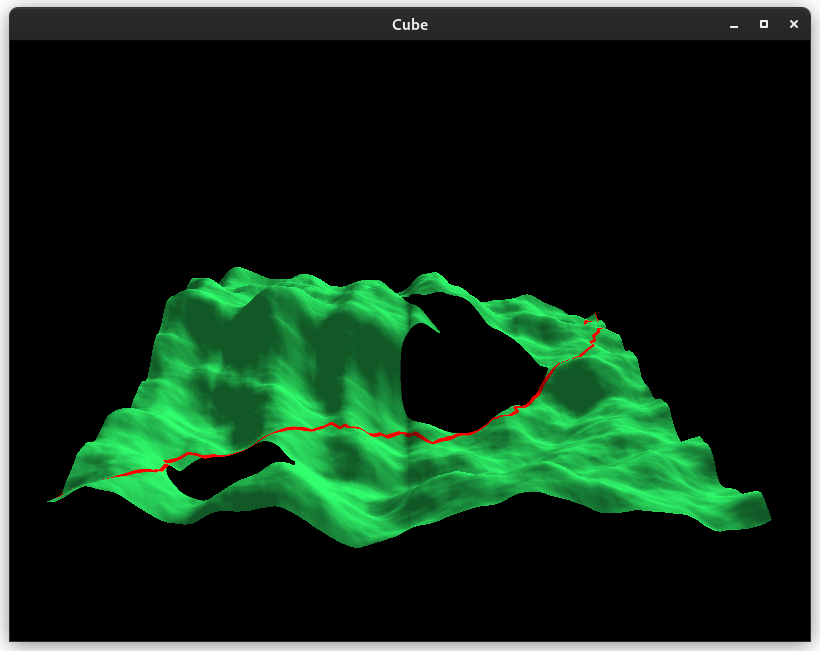
\includegraphics[scale=0.18]{content/dijkstra.png}
            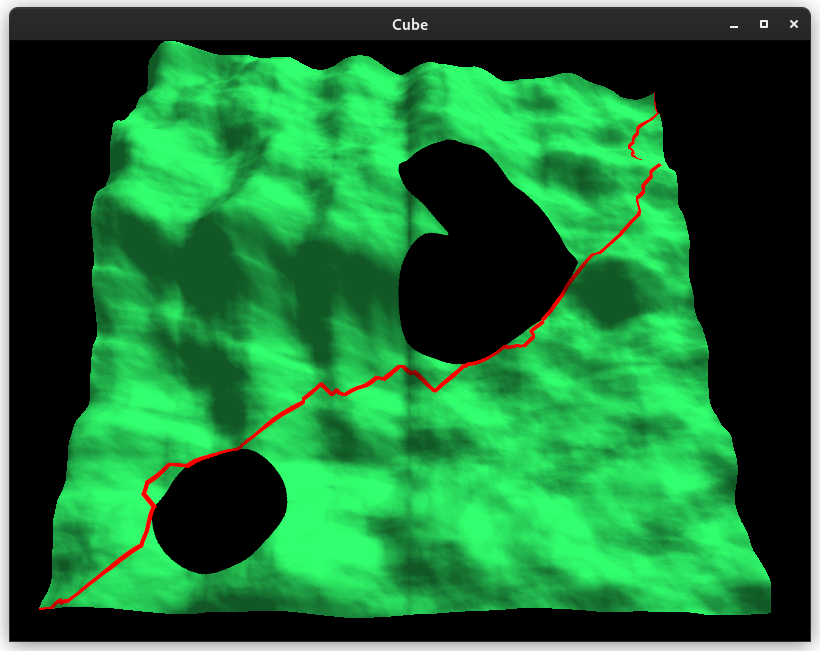
\includegraphics[scale=0.18]{content/dijkstra-top.png}
        \end{center}
        Время перехода
        \[
            d_{i,j}(\hat i, \hat j) = 100\cdot(\mathrm{height}(\hat i, \hat j) - \mathrm{height}(i, j))_{+} + 5.
        \]
    \end{frame}
    \begin{frame}[t]{Пример 2}
        Алгоритм Беллмана--Форда из $(1,\,1)$ в $(90,\,90)$
        \begin{center}
            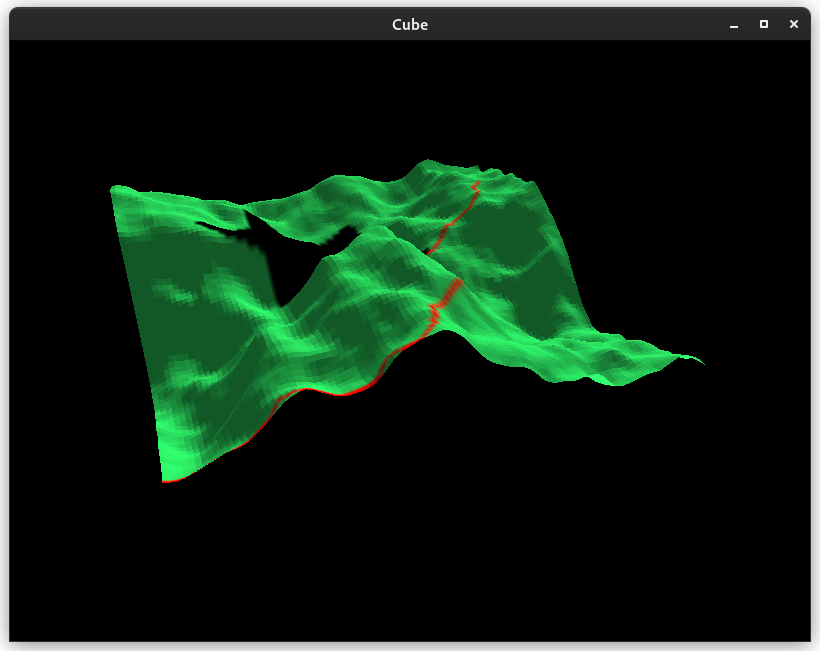
\includegraphics[scale=0.18]{content/bf.png}
            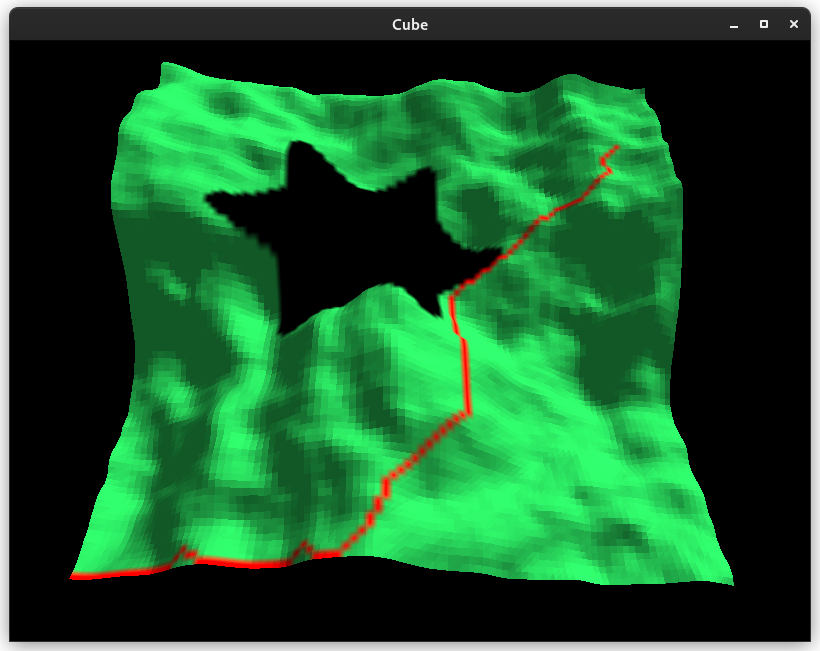
\includegraphics[scale=0.18]{content/bf-top.png}
        \end{center}
        Время перехода
        \[
            d_{i,j}(\hat i, \hat j) = 100\cdot(\mathrm{height}(\hat i, \hat j) - \mathrm{height}(i, j))_{+} + 5.
        \]
    \end{frame}
    \begin{frame}[t]{Сравнение времени работы}
        Время работы алгоритма Беллмана--Форда
            \begin{tabular}{ | l | l | l | l |}
                \hline
                Сетка   & Классический    & Парал. однонод. & Парал. многонод. \\ \hline
                50$\times$50   & 2s              & 700ms             & 2s                 \\
                100$\times$100 & 28s             & 11s               & 24s                \\
                250$\times$250 & 14m 17s         & 4m 56s            & 10m 24s             \\
                500$\times$500 & $\approx$4h 50m & $\approx$1h 20m   & $\approx$2h 40m    \\
                \hline
            \end{tabular}
        \vfill 
        Время работы алгоритма Дейкстры
            \begin{tabular}{ | l | l | l | l |}
                \hline
                Сетка     & Классический    & Парал. однонод. & Парал. многонод. \\ \hline
                500$\times$500   & 2.9             & 4.5s              & 19.4s               \\
                1000$\times$1000 & 36s             & 40s               & 3m 20s             \\
                2500$\times$2500 & 10m 40s         & 6m 48s            & 34m 42s            \\
                5000$\times$5000 & $\approx$1h 15m & $\approx$39m      & $\approx$2h 40m    \\
                \hline
            \end{tabular}
    \end{frame}
    \begin{frame}[t]{Литература}
        \begin{enumerate}
            \item Беллман~Р., Дрейфус~С. \textit{Прикладные задачи динамического программирования.} М.:~Наука,~1965.
            \item Shu-Xi, Wang. \textit{The Improved Dijkstra's Shortest Path Algorithm and Its Application.} Procedia Engineering. 29. 1186-1190. 2012.
            \item Glabowski, M., Musznicki, B. \textit{Review and Performance Analysis of Shortest Path Problem Solving Algorithms.} International Journal On Advances in Software. 7. 20-30. 2014.
            \item Ведякова А. О., Милованович Е. В. \textit{Методы теории оптимального управления.} М.: Редакционно-издательский отдел Университета ИТМО. Санкт-Петербург, 2021.
        \end{enumerate}
    \end{frame}
\end{document}

\usepackage{adjustbox}
\usepackage{amsfonts}
\title[Курсовая работа]
    {Построение параллельных алгоритмов для решения задачи быстродействия с фазовыми ограничениями}
\author[К. Ю. Егоров]
    {студент 5 курса К. Ю. Егоров\\
    научный руководитель --- к.ф-м.н., доцент И. В. Востриков}
\institute{Кафедра системного анализа}
\date{28 мая 2022 г.}

\begin{document}
    \maketitle
    \begin{frame}[t]{Постановка задачи}
        Рассмотрим задачу
        \begin{equation*}
            \dot x = f(t,x,u),\;\mbox{где $x = [x_1, x_2, \dot x_1, \dot x_2]$.}
        \end{equation*}
        Фазовые ограничения
        \begin{equation*}
            [x_1, x_2] \in \Omega \subseteq \mathbb{R}^2.
        \end{equation*}
        Минимизируем функционал
        \begin{equation*}
            J(u) = \int_{t_0}^{t_1}g(x, u)\,dt \to \min_u.
        \end{equation*}
        Необходимо решать уравнение Гамильтона--Якоби--Беллмана
        \begin{equation*}
            \min\limits_{u \in U}\left\{
                g(x,u) + \sum\limits_{i=1}^{n}\frac{\partial V(x)}{\partial x_i} f_i(x,u)
            \right\} = 0.
        \end{equation*}
    \end{frame}
    \begin{frame}[t]{Дискретизация задачи}
        Введем равномерную сетку
        \begin{equation*}
            \Xi = \left\{ (x_i , y_j) \in \Pi , x_i = \varepsilon\frac{i}{N} , y_j = \varepsilon\frac{j}{M} \right\},\,
            \mbox{где $\Omega \subseteq \Pi$}.
        \end{equation*}
        Возможные переходы для $(i,j)$
        \begin{equation*}
            \mathrm{possible}(i,j) = \{
                (i, j) \;|\; i \in \{i, i \pm 1\}, j \in \{j, j \pm 1\}, (x_i,y_j) \in \Omega    
            \}
        \end{equation*}
        \textit{Предложение.} Время перехода не зависит от предыдущей скорости и направления. Обозначим это время за
        \begin{equation*}
            d_{i_{from},\,j_{from}}(i_{to},\,j_{to}).
        \end{equation*}
        Неявное матричное уравнение
        \begin{equation*}
            \begin{aligned}
                &V_{i,j} = \min\limits_{(\hat i,\,\hat j) \in \mathrm{possible}(i,\,j)}\{d_{i,\,j}(\hat i,\,\hat j) + V_{\hat i,\,\hat j}\}, \\
                &V_{i_1,\,j_1} = 0.
            \end{aligned}
        \end{equation*}
    \end{frame}
    \begin{frame}[t]{Алгоритм Беллмана--Форда}
        \begin{enumerate}
            \item Изначально все узлы, кроме целевого, промаркированы значением $+\infty$, а целевой~--- нулем;
            \item Необходимо провести $(NM - 1)$ итерации алгоритма;
            \item На каждой итерации происходит полный проход по сетке, далее $(i,j)$ --- позиция при проходе;
            \item Для каждой вершины из возможного множества $(\hat i, \hat j) \in \mathrm{possible}(i,j)$ происходит перемаркировка: в случае, если $V(i, j) > d_{i,j}(\hat i, \hat j) + V(\hat i, \hat j)$, перемаркируем
            \[
                V(i,j) \leftarrowtail d_{i,j}(\hat i, \hat j) + V(\hat i, \hat j).
            \]
        \end{enumerate}
        \begin{block}{Замечание}
            Оптимальная траектория не может иметь более $(NM - 1)$ перемещения. Таким образом алгоритм действительно ищет кратчайший путь.
        \end{block}
    \end{frame}
    \begin{frame}[t]{Параллельный алгоритм Беллмана--Форда}
        На центральном процессоре
        \begin{itemize}
            \item Разбиваем сетку на каждой итерации на $C$ (число ядер) подсеток, считающихся параллельно
            \item Синхронизацию при обработке последнего ряда подсетки осуществляем массивом мьютексов
        \end{itemize}
        На графическом процессоре
        \begin{itemize}
            \item Каждый узел считается на отдельном процессоре
            \item Синхронизация осуществляется за счет того, что проводится не один проход по матрице, а восемь: отдельно для каждого возможного направления движения
        \end{itemize}
        На многонодной установке
        \begin{itemize}
            \item Одна мастер программа, $LC_l$ (совокупное число ядер) вычислителей (сервисов, общающихся по http)
            \item Синхронизация осуществляется за счет передачи мастером минимального инкремента каждому вычислителю
        \end{itemize}
    \end{frame}
    \begin{frame}[t]{Алгоритм Дейкстры}
        \begin{enumerate}
            \item На начало алгоритма в множестве граничных узлов находится только целевой узел. 
            \item На каждой итерации алгоритма из множества граничных узлов выбирается узел с минимальной маркировкой.
            \item Этот узел добавляется в множество обработанных узлов и удаляется из граничного множества.
            \item Затем из возможного множества выбираются узлы, которые не находятся в множестве обработанных узлов. Эти узлы добавляются в множество граничных вершин, маркировка таких вершин обновляется.
        \end{enumerate}
        Алгоритм останавливается в случае, если на некоторой итерации алгоритма был выбран начальный узел $(i_0,j_0)$.
    \end{frame}
    \begin{frame}[t]{Параллельный алгоритм Дейкстры}
        Распараллеливанию подвергается самый алгоритмически сложная часть алгоритма~--- поиск минимума в граничном множестве. Для этого граничное множество представляется в виде $C$ (число доступных ядер процессора) хэш-таблиц. Запись нового узла осуществляется в наименее полную таблицу.

        \begin{itemize}
            \item Для программы на центральном процессоре не требуется дополнительная синхронизация;
            \item Нет нативного метода, который мог бы поддержать графический процессор, так как взаимодействие с ним осуществляется копированием последовательных страниц памяти. Это потребовало бы использование массива для хранения граничного множества, и в конечном итоге ускорение было бы скомпенсировано операцией удаления из массива;
            \item Для многонодной установки минимальная инкрементальная информация~--- это выбранный узел, и узлы, добавленные в граничное множество.
        \end{itemize}
    \end{frame}
    \begin{frame}[t]{Программное решение}
        Программы написаны на языке Go
        \begin{itemize}
            \item go routines;
            \item компилируемый;
            \item сборка мусора.
        \end{itemize}
        Помимо основных алгоритмов написаны:
        \begin{itemize}
            \item генератор ландшафта, использующий перлиновый шум;
            \item визуализатор пути, использующий OpenGL.
        \end{itemize}
        Программы для многонодной установки
        \begin{itemize}
            \item поставляются в виде двух docker-образов: для мастера и вычислителе;.
            \item тестировалось только на Kubernetes кластере;
            \item требуют ручного применения Kubernetes манифестов.
        \end{itemize}
    \end{frame}
    \begin{frame}[t]{Пример 1}
        Алгоритм Дейкстры из $(1,\,1)$ в $(1000,\,1000)$
        \begin{center}
            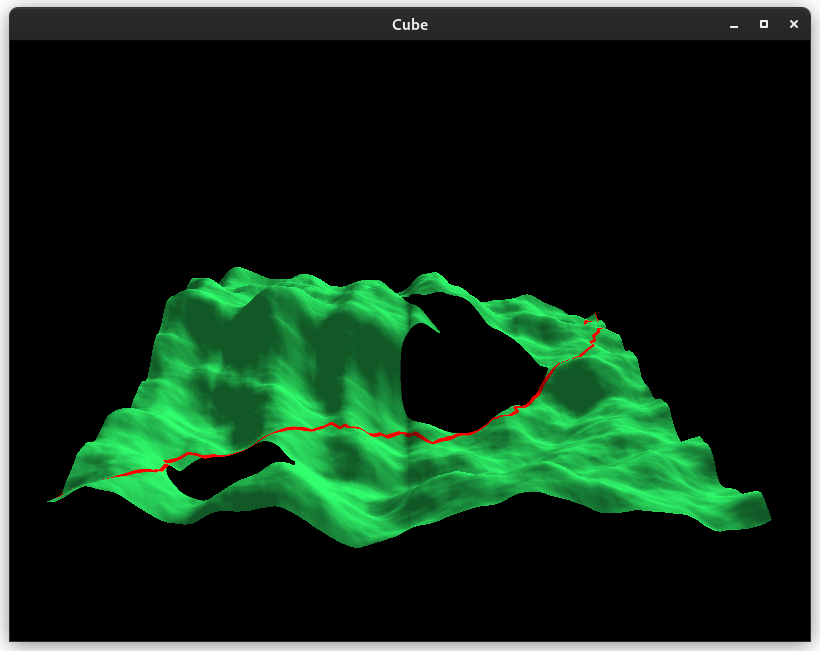
\includegraphics[scale=0.18]{content/dijkstra.png}
            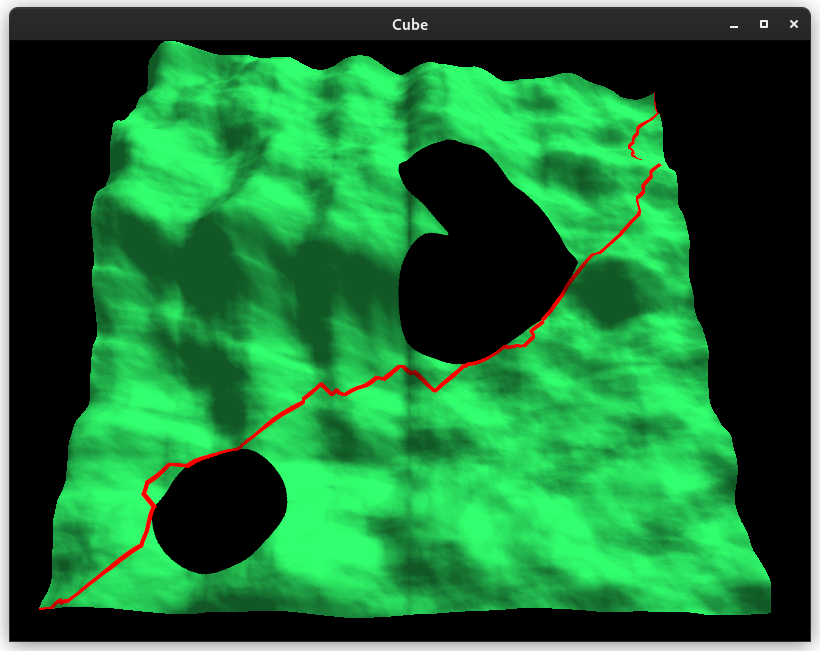
\includegraphics[scale=0.18]{content/dijkstra-top.png}
        \end{center}
        Время перехода
        \[
            d_{i,j}(\hat i, \hat j) = 100\cdot(\mathrm{height}(\hat i, \hat j) - \mathrm{height}(i, j))_{+} + 5.
        \]
    \end{frame}
    \begin{frame}[t]{Пример 2}
        Алгоритм Беллмана--Форда из $(1,\,1)$ в $(90,\,90)$
        \begin{center}
            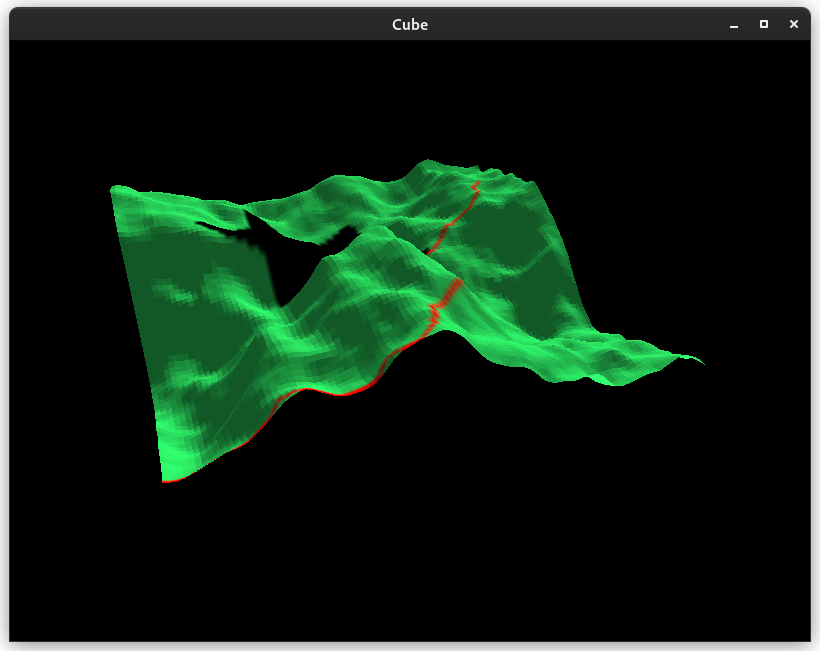
\includegraphics[scale=0.18]{content/bf.png}
            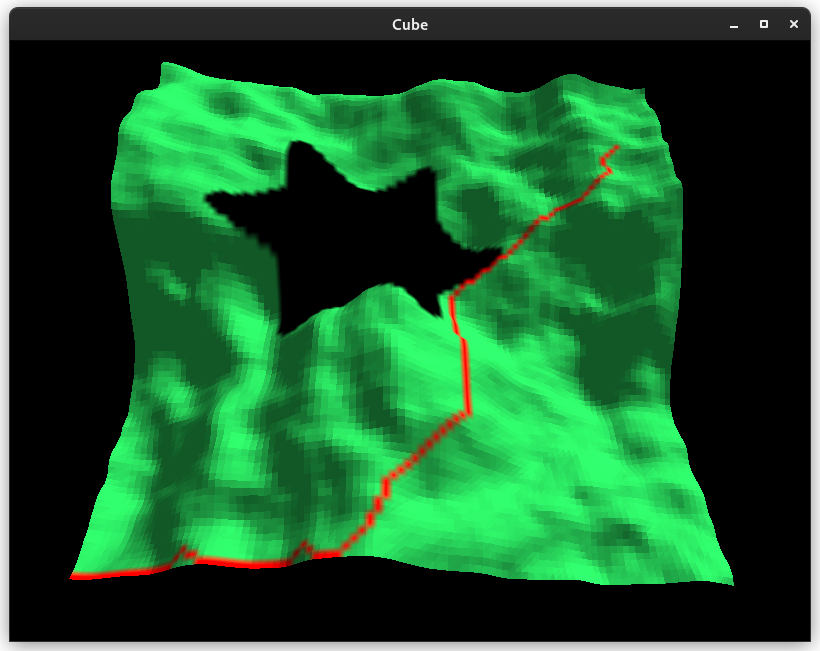
\includegraphics[scale=0.18]{content/bf-top.png}
        \end{center}
        Время перехода
        \[
            d_{i,j}(\hat i, \hat j) = 100\cdot(\mathrm{height}(\hat i, \hat j) - \mathrm{height}(i, j))_{+} + 5.
        \]
    \end{frame}
    \begin{frame}[t]{Сравнение времени работы}
        Время работы алгоритма Беллмана--Форда
            \begin{tabular}{ | l | l | l | l |}
                \hline
                Сетка   & Классический    & Парал. однонод. & Парал. многонод. \\ \hline
                50$\times$50   & 2s              & 700ms             & 2s                 \\
                100$\times$100 & 28s             & 11s               & 24s                \\
                250$\times$250 & 14m 17s         & 4m 56s            & 10m 24s             \\
                500$\times$500 & $\approx$4h 50m & $\approx$1h 20m   & $\approx$2h 40m    \\
                \hline
            \end{tabular}
        \vfill 
        Время работы алгоритма Дейкстры
            \begin{tabular}{ | l | l | l | l |}
                \hline
                Сетка     & Классический    & Парал. однонод. & Парал. многонод. \\ \hline
                500$\times$500   & 2.9             & 4.5s              & 19.4s               \\
                1000$\times$1000 & 36s             & 40s               & 3m 20s             \\
                2500$\times$2500 & 10m 40s         & 6m 48s            & 34m 42s            \\
                5000$\times$5000 & $\approx$1h 15m & $\approx$39m      & $\approx$2h 40m    \\
                \hline
            \end{tabular}
    \end{frame}
    \begin{frame}[t]{Литература}
        \begin{enumerate}
            \item Беллман~Р., Дрейфус~С. \textit{Прикладные задачи динамического программирования.} М.:~Наука,~1965.
            \item Shu-Xi, Wang. \textit{The Improved Dijkstra's Shortest Path Algorithm and Its Application.} Procedia Engineering. 29. 1186-1190. 2012.
            \item Glabowski, M., Musznicki, B. \textit{Review and Performance Analysis of Shortest Path Problem Solving Algorithms.} International Journal On Advances in Software. 7. 20-30. 2014.
            \item Ведякова А. О., Милованович Е. В. \textit{Методы теории оптимального управления.} М.: Редакционно-издательский отдел Университета ИТМО. Санкт-Петербург, 2021.
        \end{enumerate}
    \end{frame}
\end{document}